\documentclass[final,t,serif]{beamer}\usepackage[]{graphicx}\usepackage[]{color}
%% maxwidth is the original width if it is less than linewidth
%% otherwise use linewidth (to make sure the graphics do not exceed the margin)
\makeatletter
\def\maxwidth{ %
  \ifdim\Gin@nat@width>\linewidth
    \linewidth
  \else
    \Gin@nat@width
  \fi
}
\makeatother

\definecolor{fgcolor}{rgb}{0.345, 0.345, 0.345}
\newcommand{\hlnum}[1]{\textcolor[rgb]{0.686,0.059,0.569}{#1}}%
\newcommand{\hlstr}[1]{\textcolor[rgb]{0.192,0.494,0.8}{#1}}%
\newcommand{\hlcom}[1]{\textcolor[rgb]{0.678,0.584,0.686}{\textit{#1}}}%
\newcommand{\hlopt}[1]{\textcolor[rgb]{0,0,0}{#1}}%
\newcommand{\hlstd}[1]{\textcolor[rgb]{0.345,0.345,0.345}{#1}}%
\newcommand{\hlkwa}[1]{\textcolor[rgb]{0.161,0.373,0.58}{\textbf{#1}}}%
\newcommand{\hlkwb}[1]{\textcolor[rgb]{0.69,0.353,0.396}{#1}}%
\newcommand{\hlkwc}[1]{\textcolor[rgb]{0.333,0.667,0.333}{#1}}%
\newcommand{\hlkwd}[1]{\textcolor[rgb]{0.737,0.353,0.396}{\textbf{#1}}}%

\usepackage{framed}
\makeatletter
\newenvironment{kframe}{%
 \def\at@end@of@kframe{}%
 \ifinner\ifhmode%
  \def\at@end@of@kframe{\end{minipage}}%
  \begin{minipage}{\columnwidth}%
 \fi\fi%
 \def\FrameCommand##1{\hskip\@totalleftmargin \hskip-\fboxsep
 \colorbox{shadecolor}{##1}\hskip-\fboxsep
     % There is no \\@totalrightmargin, so:
     \hskip-\linewidth \hskip-\@totalleftmargin \hskip\columnwidth}%
 \MakeFramed {\advance\hsize-\width
   \@totalleftmargin\z@ \linewidth\hsize
   \@setminipage}}%
 {\par\unskip\endMakeFramed%
 \at@end@of@kframe}
\makeatother

\definecolor{shadecolor}{rgb}{.97, .97, .97}
\definecolor{messagecolor}{rgb}{0, 0, 0}
\definecolor{warningcolor}{rgb}{1, 0, 1}
\definecolor{errorcolor}{rgb}{1, 0, 0}
\newenvironment{knitrout}{}{} % an empty environment to be redefined in TeX

\usepackage{alltt}
\mode<presentation>
{
%  \usetheme{Warsaw}
%  \usetheme{Aachen}
%  \usetheme{Oldi6}
%  \usetheme{I6td}
  \usetheme{I6dv}
%  \usetheme{I6pd}
%  \usetheme{I6pd2}
}
% additional settings
\setbeamerfont{itemize}{size=\normalsize}
\setbeamerfont{itemize/enumerate body}{size=\normalsize}
\setbeamerfont{itemize/enumerate subbody}{size=\normalsize}

% additional packages
\usepackage{xcolor}
\usepackage{amsmath,amsthm, amssymb, latexsym}
\usepackage{exscale}
\usepackage{subfig}
%\boldmath
\usepackage{booktabs, array}
\usepackage{tabularx}
%\usepackage{rotating} %sideways environment
\usepackage[english]{babel}
\usepackage[latin1]{inputenc}
\usepackage{times}
\usepackage[orientation=landscape,size=custom,width=115.57,height=99.695,scale=1.55]{beamerposter} % in cm, equal to 45.5" wide x 39.3701" high
\listfiles
% Display a grid to help align images
%\beamertemplategridbackground[1cm]

\newcolumntype{R}{>{\raggedleft\arraybackslash}X}

% for lining up blocks within a column to a single block/column above
% http://tex.stackexchange.com/questions/74808/how-to-line-up-blocks-in-columns-with-full-width-blocks-in-beamer-beamerposter
\newenvironment<>{varblock}[2][.9\textwidth]{%
  \setlength{\textwidth}{#1}
  \begin{actionenv}#3%
    \def\insertblocktitle{#2}%
    \par%
    \usebeamertemplate{block begin}}
  {\par%
    \usebeamertemplate{block end}%
  \end{actionenv}}

\title{\LARGE Four Decades of Water Quality Changes in the Upper San Francisco Estuary}
\author[Beck et al.]{Marcus W. Beck\textsuperscript{1}, David Senn\textsuperscript{2}, Emily Novick\textsuperscript{2}, Phil Bresnahan\textsuperscript{2}, James D. Hagy III\textsuperscript{1}, Thomas Jabusch\textsuperscript{2}}
\institute[USEPA GED]{\textsuperscript{1}US Environmental Protection Agency ORD NHEERL, Gulf Ecology Division, Gulf Breeze, FL\\\textsuperscript{2}San Francisco Estuary Institute, Richmond, CA}
\date[April 20, 2016]{April 20, 2016}



\IfFileExists{upquote.sty}{\usepackage{upquote}}{}
\begin{document}

\begin{frame}{}

	\vspace{-1cm} %spacing for block distance from header
  \begin{columns}[t]
  	\hspace{0.4cm}
  	
  	%%%%%%%%%%%%%%
  	% LEFT
  	%%%%%%%%%%%%%%
  	\begin{column}{.31\linewidth}

			%%%%%%
			% abstract
			%%%%%%
      \begin{block}{Abstract}
        		\alert{\small Recent methods for trend analysis have been developed that leverage the descriptive potential of long term time series.  Combined with these methods, multi-decadal datasets of water quality in the San Francisco Estuary (SFE) could provide a valuable opportunity to gain insight into ecosystem properties and drivers of change in estuaries.  This study explores the use of an estuarine adaptation of the Weighted Regression on Time, Discharge, and Season (WRTDS) approach to describe nutrient trends in the northern region of SFE (Suisun Bay and the Delta), a primary source of nutrients into the system.  This novel technique is data-driven where the parameterization of the functional model changes smoothly over time following dynamic patterns of season and flow.  By doing so, changes over time that have not been previously quantified can be described, including variation in flow-normalized concentrations, frequency occurrence of extreme events, and response to historical changes in the watershed, all of which are important needs for understanding trends in the northern SFE.  The goal of the analysis is to apply the WRTDS model at multiple stations in the Delta and Suisun Bay regions of SFE to describe variation over time and relationships between key species of dissolved inorganic nitrogen (ammonium, nitrate/nitrite, total).  This variation is considered in the context of varying contributions of input flows from the Sacramento and San Joaquin rivers, as well as tidal exchange with the central SFE.  Overall, this analysis is expected to further an ecological and management-based understanding of dynamics in SFE, with implications for water quality restoration and protection of this prominent system.}
      \end{block}
      
      %%%%%%
      % Objectives
      %%%%%%
      \begin{block}{Analysis Components}
    	\begin{itemize}
    	\item Weighted Regressions on Time, Discharge, and Season (WRTDS) were applied to \alert{nine stations} in the upper SFE
    	\item Models were developed for \alert{three nitrogen analytes}: dissolved inorganic nitrogen (DIN), nitrite/nitrate, and ammonium
    	\item Trends were evaluated by monthly and annual periods using \alert{flow-normalized predictions} from WRTDS
    	\end{itemize}
    	
      \end{block}
      		
      %%%%%%
      % Water Quality and Flow Data
      %%%%%%

			\begin{block}{Water Quality and Flow Data}
			\begin{itemize}
	    \item Data from 1976 to 2012 for \alert{nine nutrient stations} and \alert{daily flow estimates} from major inflows were modelled
	    \end{itemize}
	    \begin{figure}
      \centerline{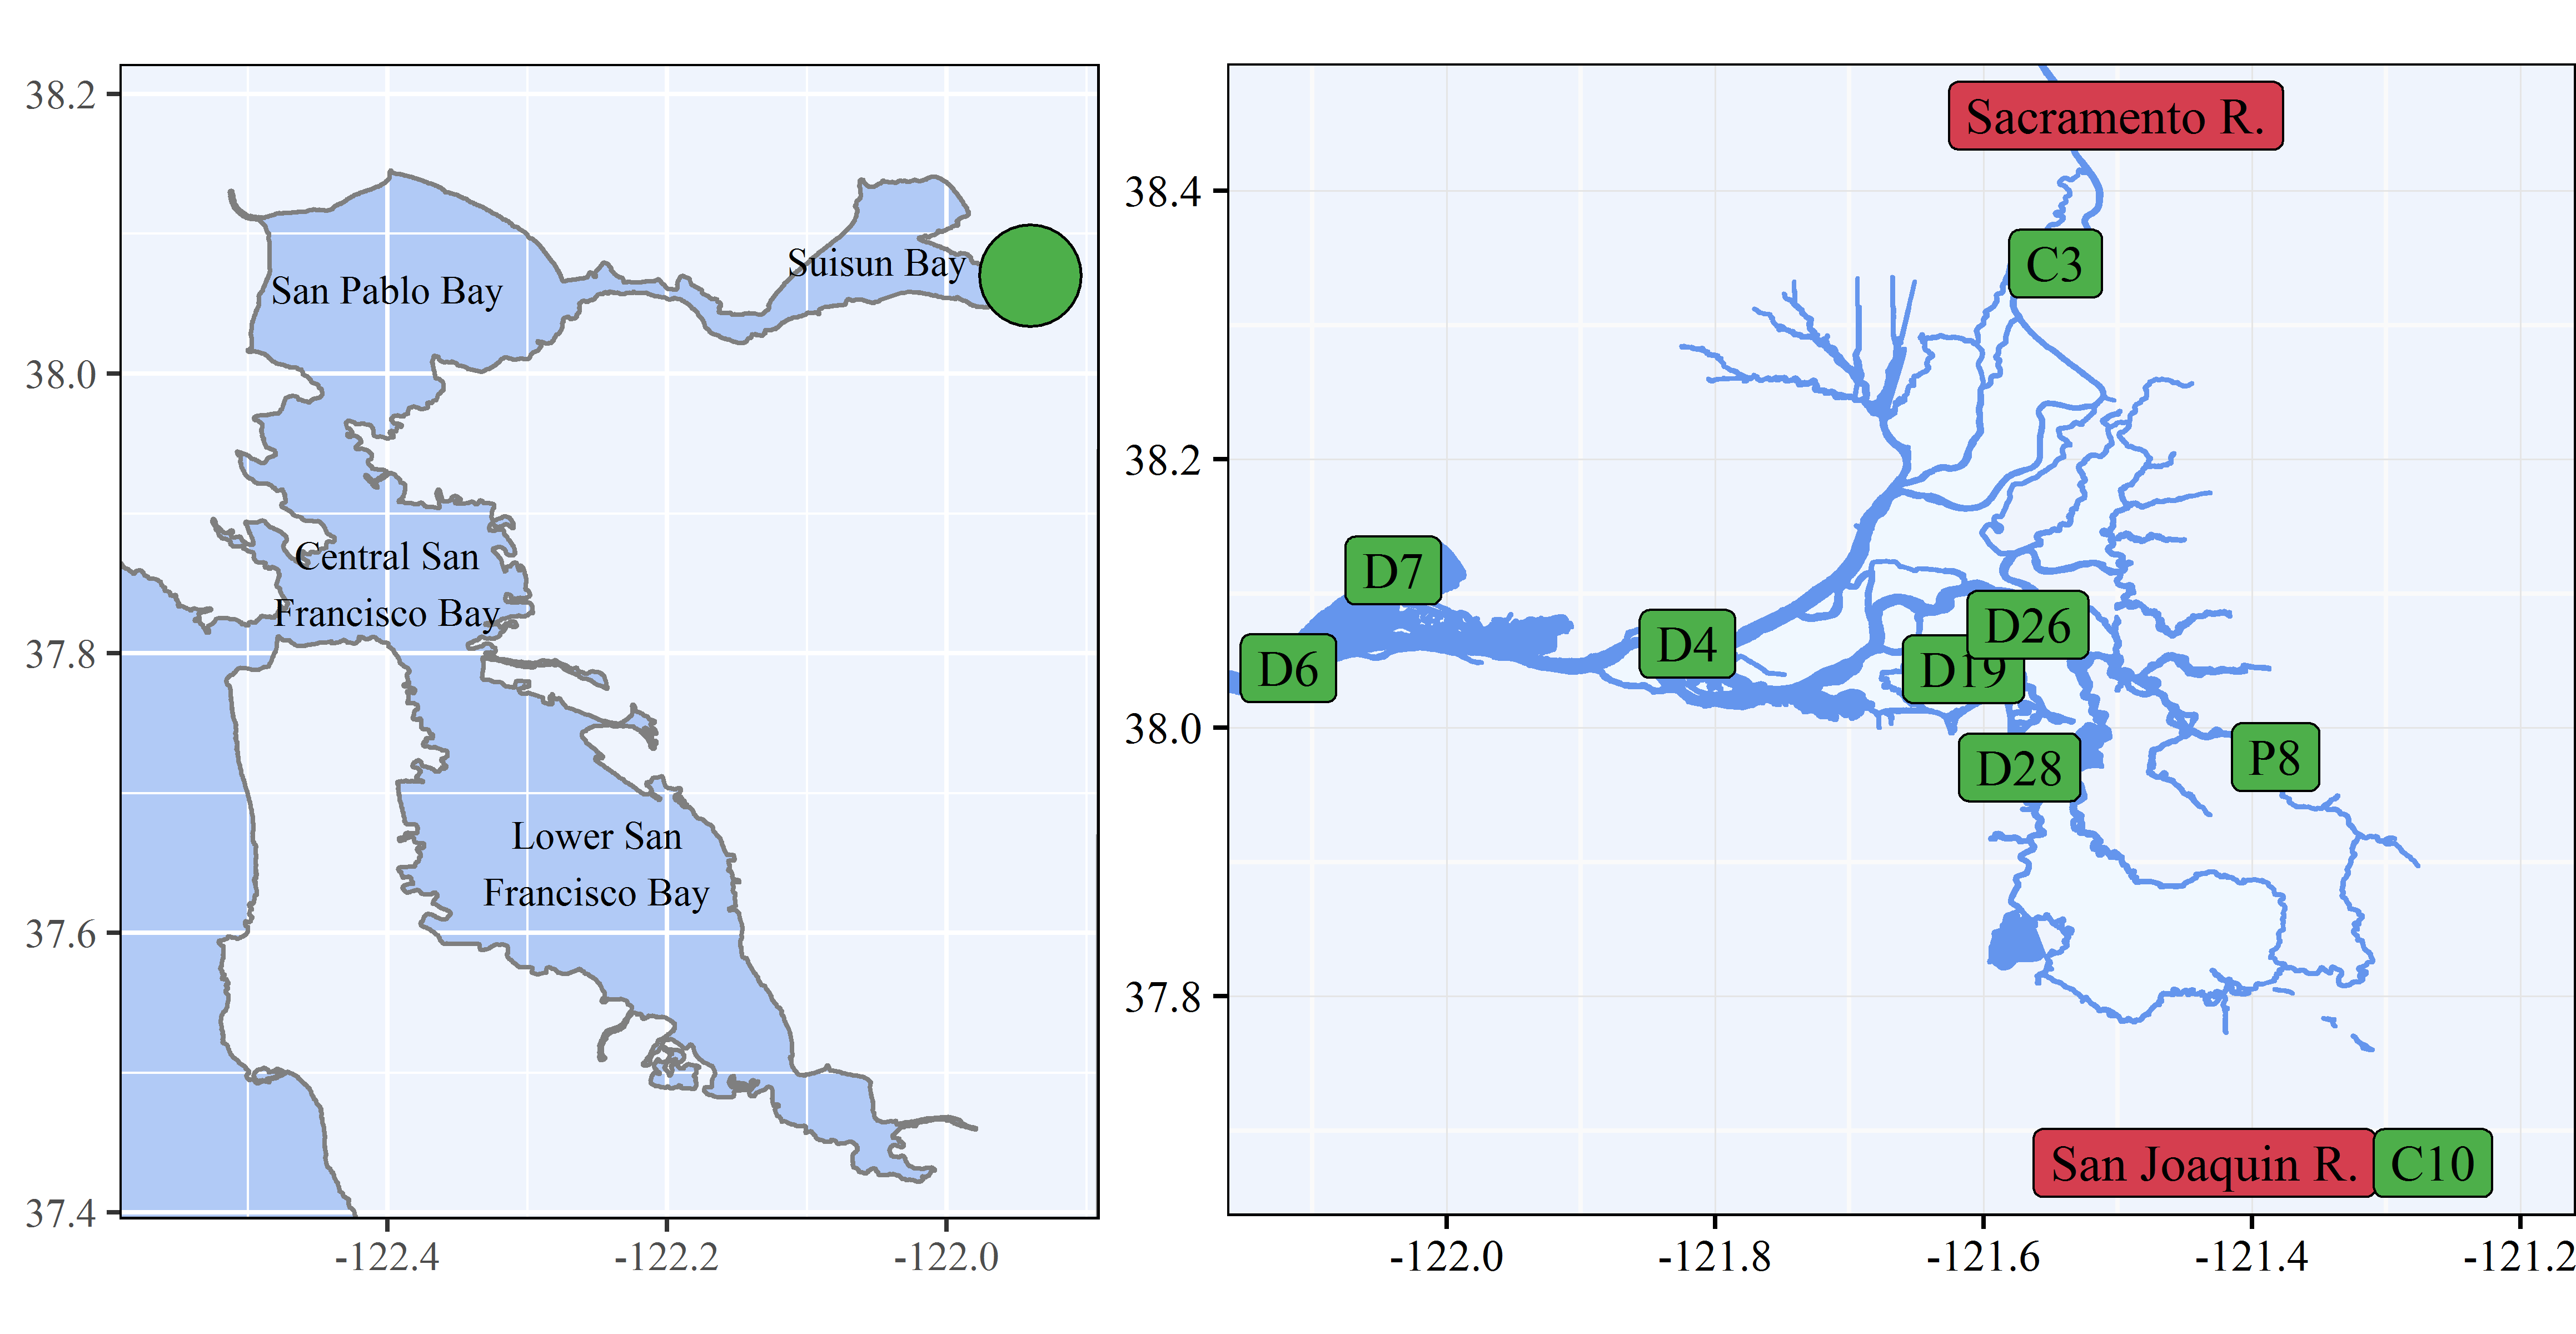
\includegraphics[width=0.95\linewidth]{posterfigs/stations.png}}
      \caption{\footnotesize Locations of bimonthly nutrient (green) and daily flow (red) stations in upper SFE.}
	    \end{figure}
	    \vspace{-2cm}
			\end{block}

    \end{column}
    
  	%%%%%%%%%%%%%%
  	% CENTER, RIGHT, TOP BLOCKS
  	%%%%%%%%%%%%%%    
    \begin{column}{.62\linewidth}

    
      %%%%%%
      % Applying Weighted Regression
      %%%%%%
      \begin{block}{Applying Weighted Regression on Time, Discharge, and Season (WRTDS)}
      
      \begin{columns}[t]
  
      %%
      \begin{column}{0.42\linewidth}
      WRTDS models were applied to \alert{nutrient} observations in relation to \alert{time, discharge, and season} 
        {\footnotesize \vspace{0.5cm}
        \centerline{$\ln\left(N\right) = \beta_0 + \beta_1 t + \beta_2 \ln\left(Q\right) + \beta_3 \sin\left(2\pi t\right) + \beta_4 \cos\left(2\pi t\right)$}
        }\vspace{-1.90cm}
  	    \begin{figure}
        \centerline{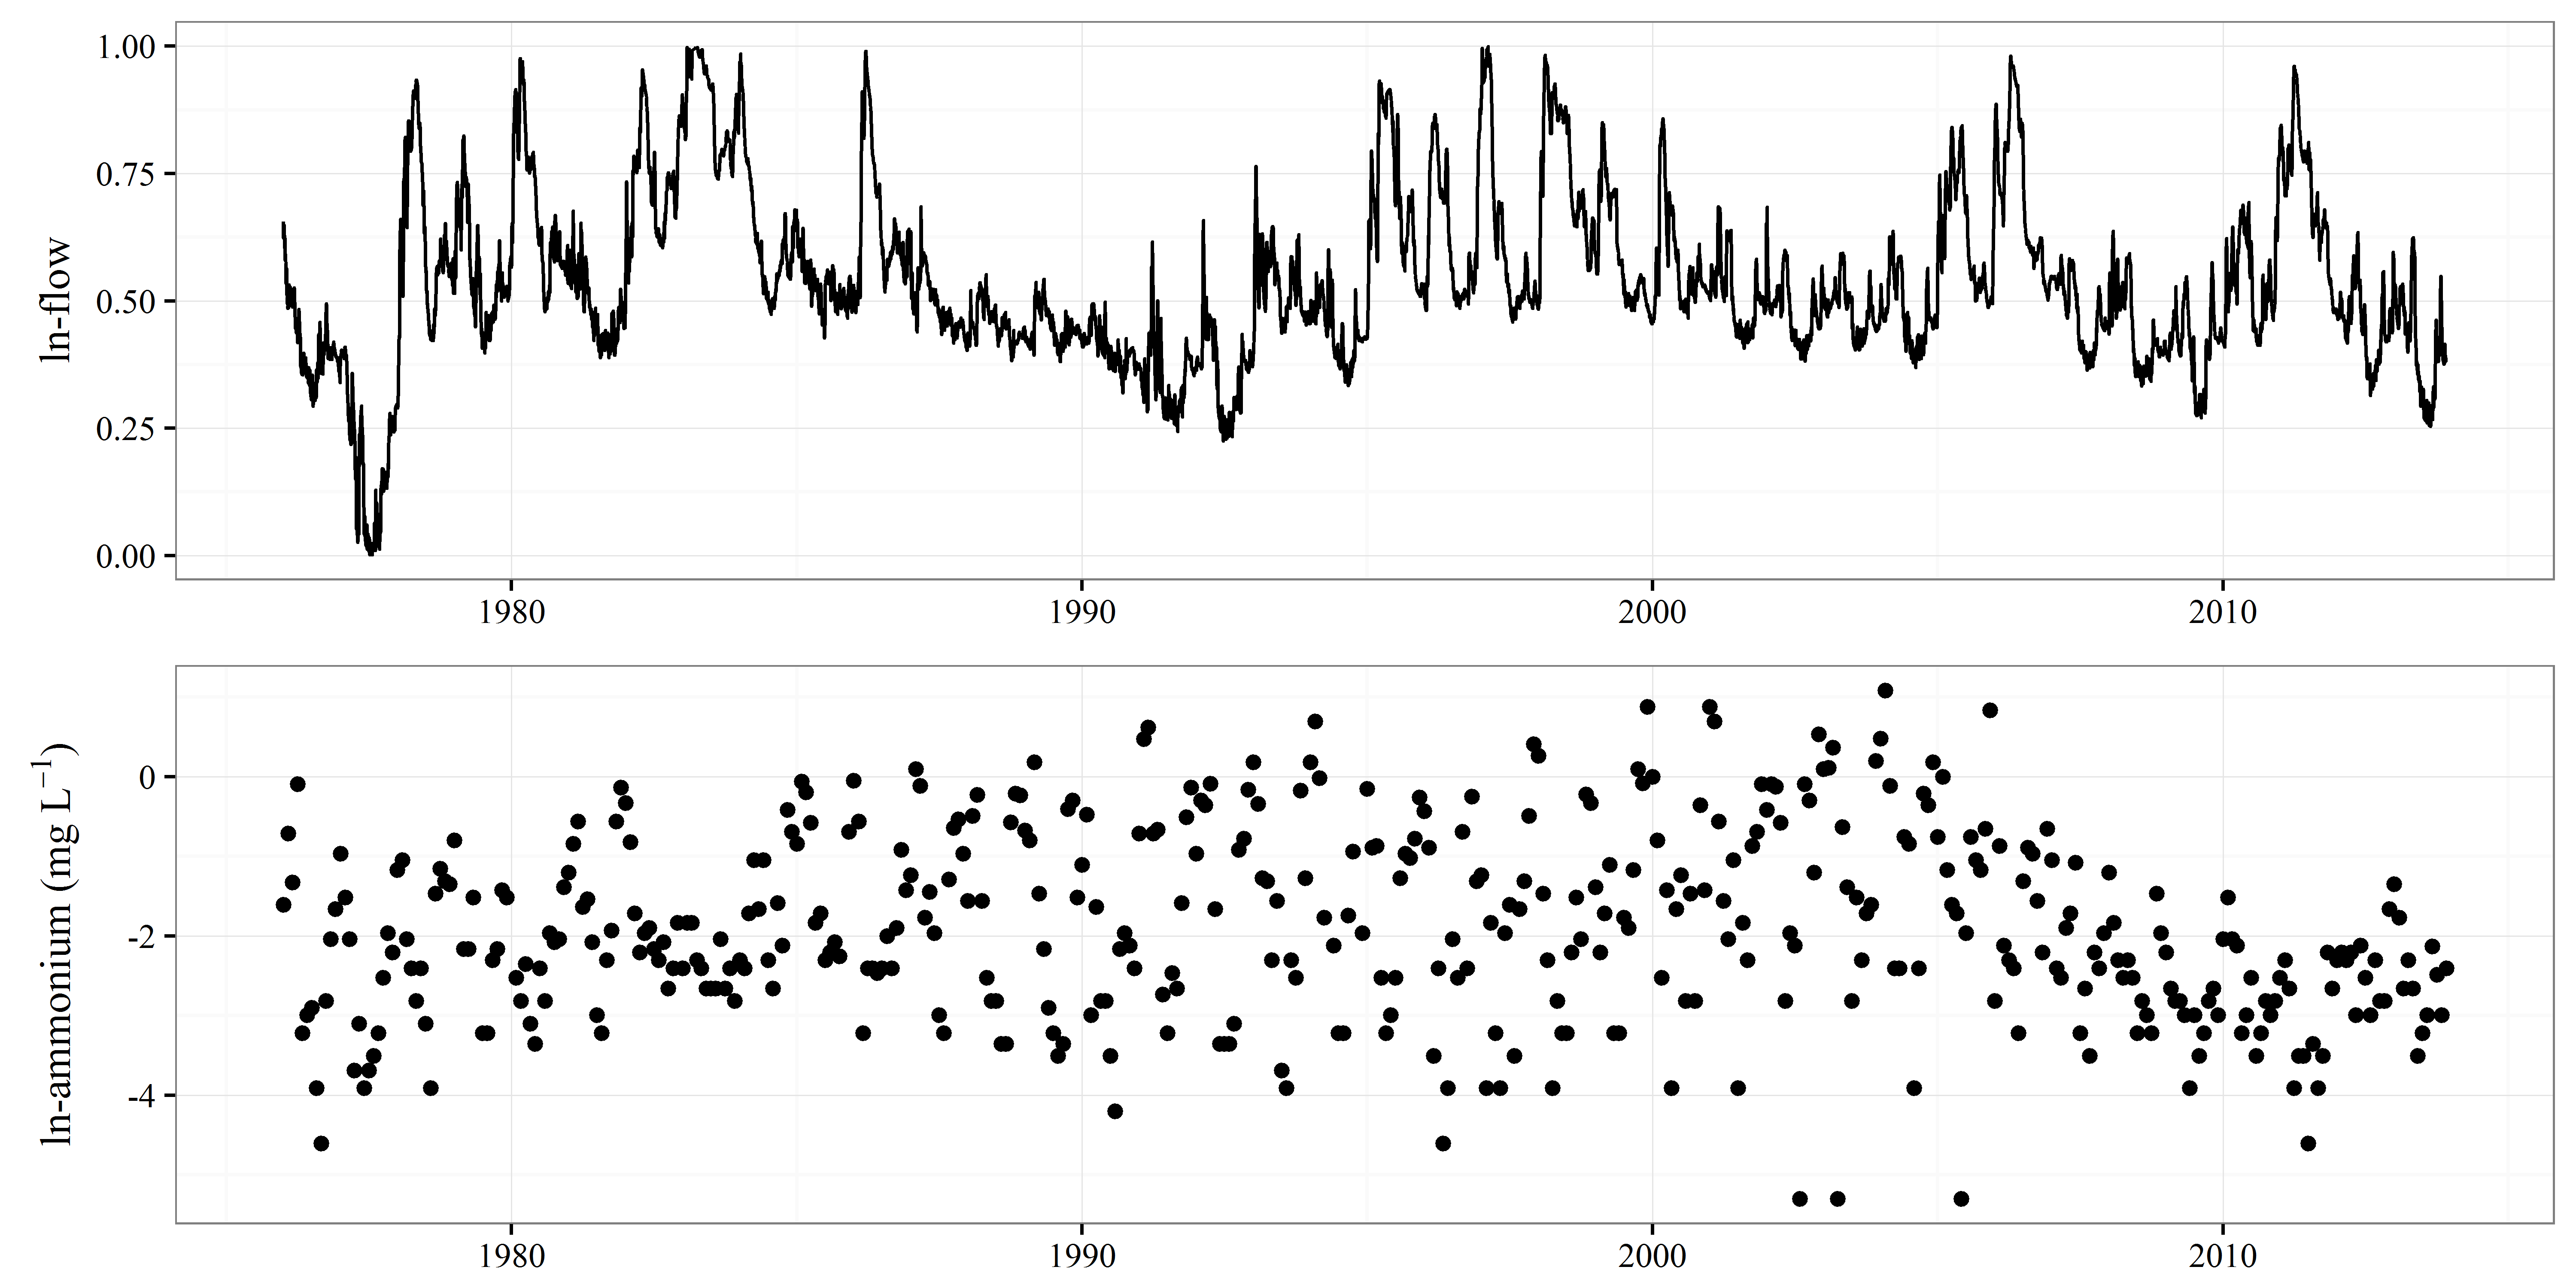
\includegraphics[width=\linewidth]{posterfigs/rawdat.png} \vspace{-0.35cm}}
        \caption{\footnotesize Example of raw flow and nitrogen data at P8 used with WRTDS.  The model was fit to matched flow and nutrient data at a bimonthly time step and then results were predicted at a daily time step.}
  	    \end{figure}		
	    
	    \end{column}
	    
	    %%
	    \begin{column}{0.53\linewidth}
	      WRTDS output showed \alert{seasonal variation}, response to \alert{flow changes}, and different \alert{conditional quantile distributions} of nutrients
	      \begin{figure}
        \centerline{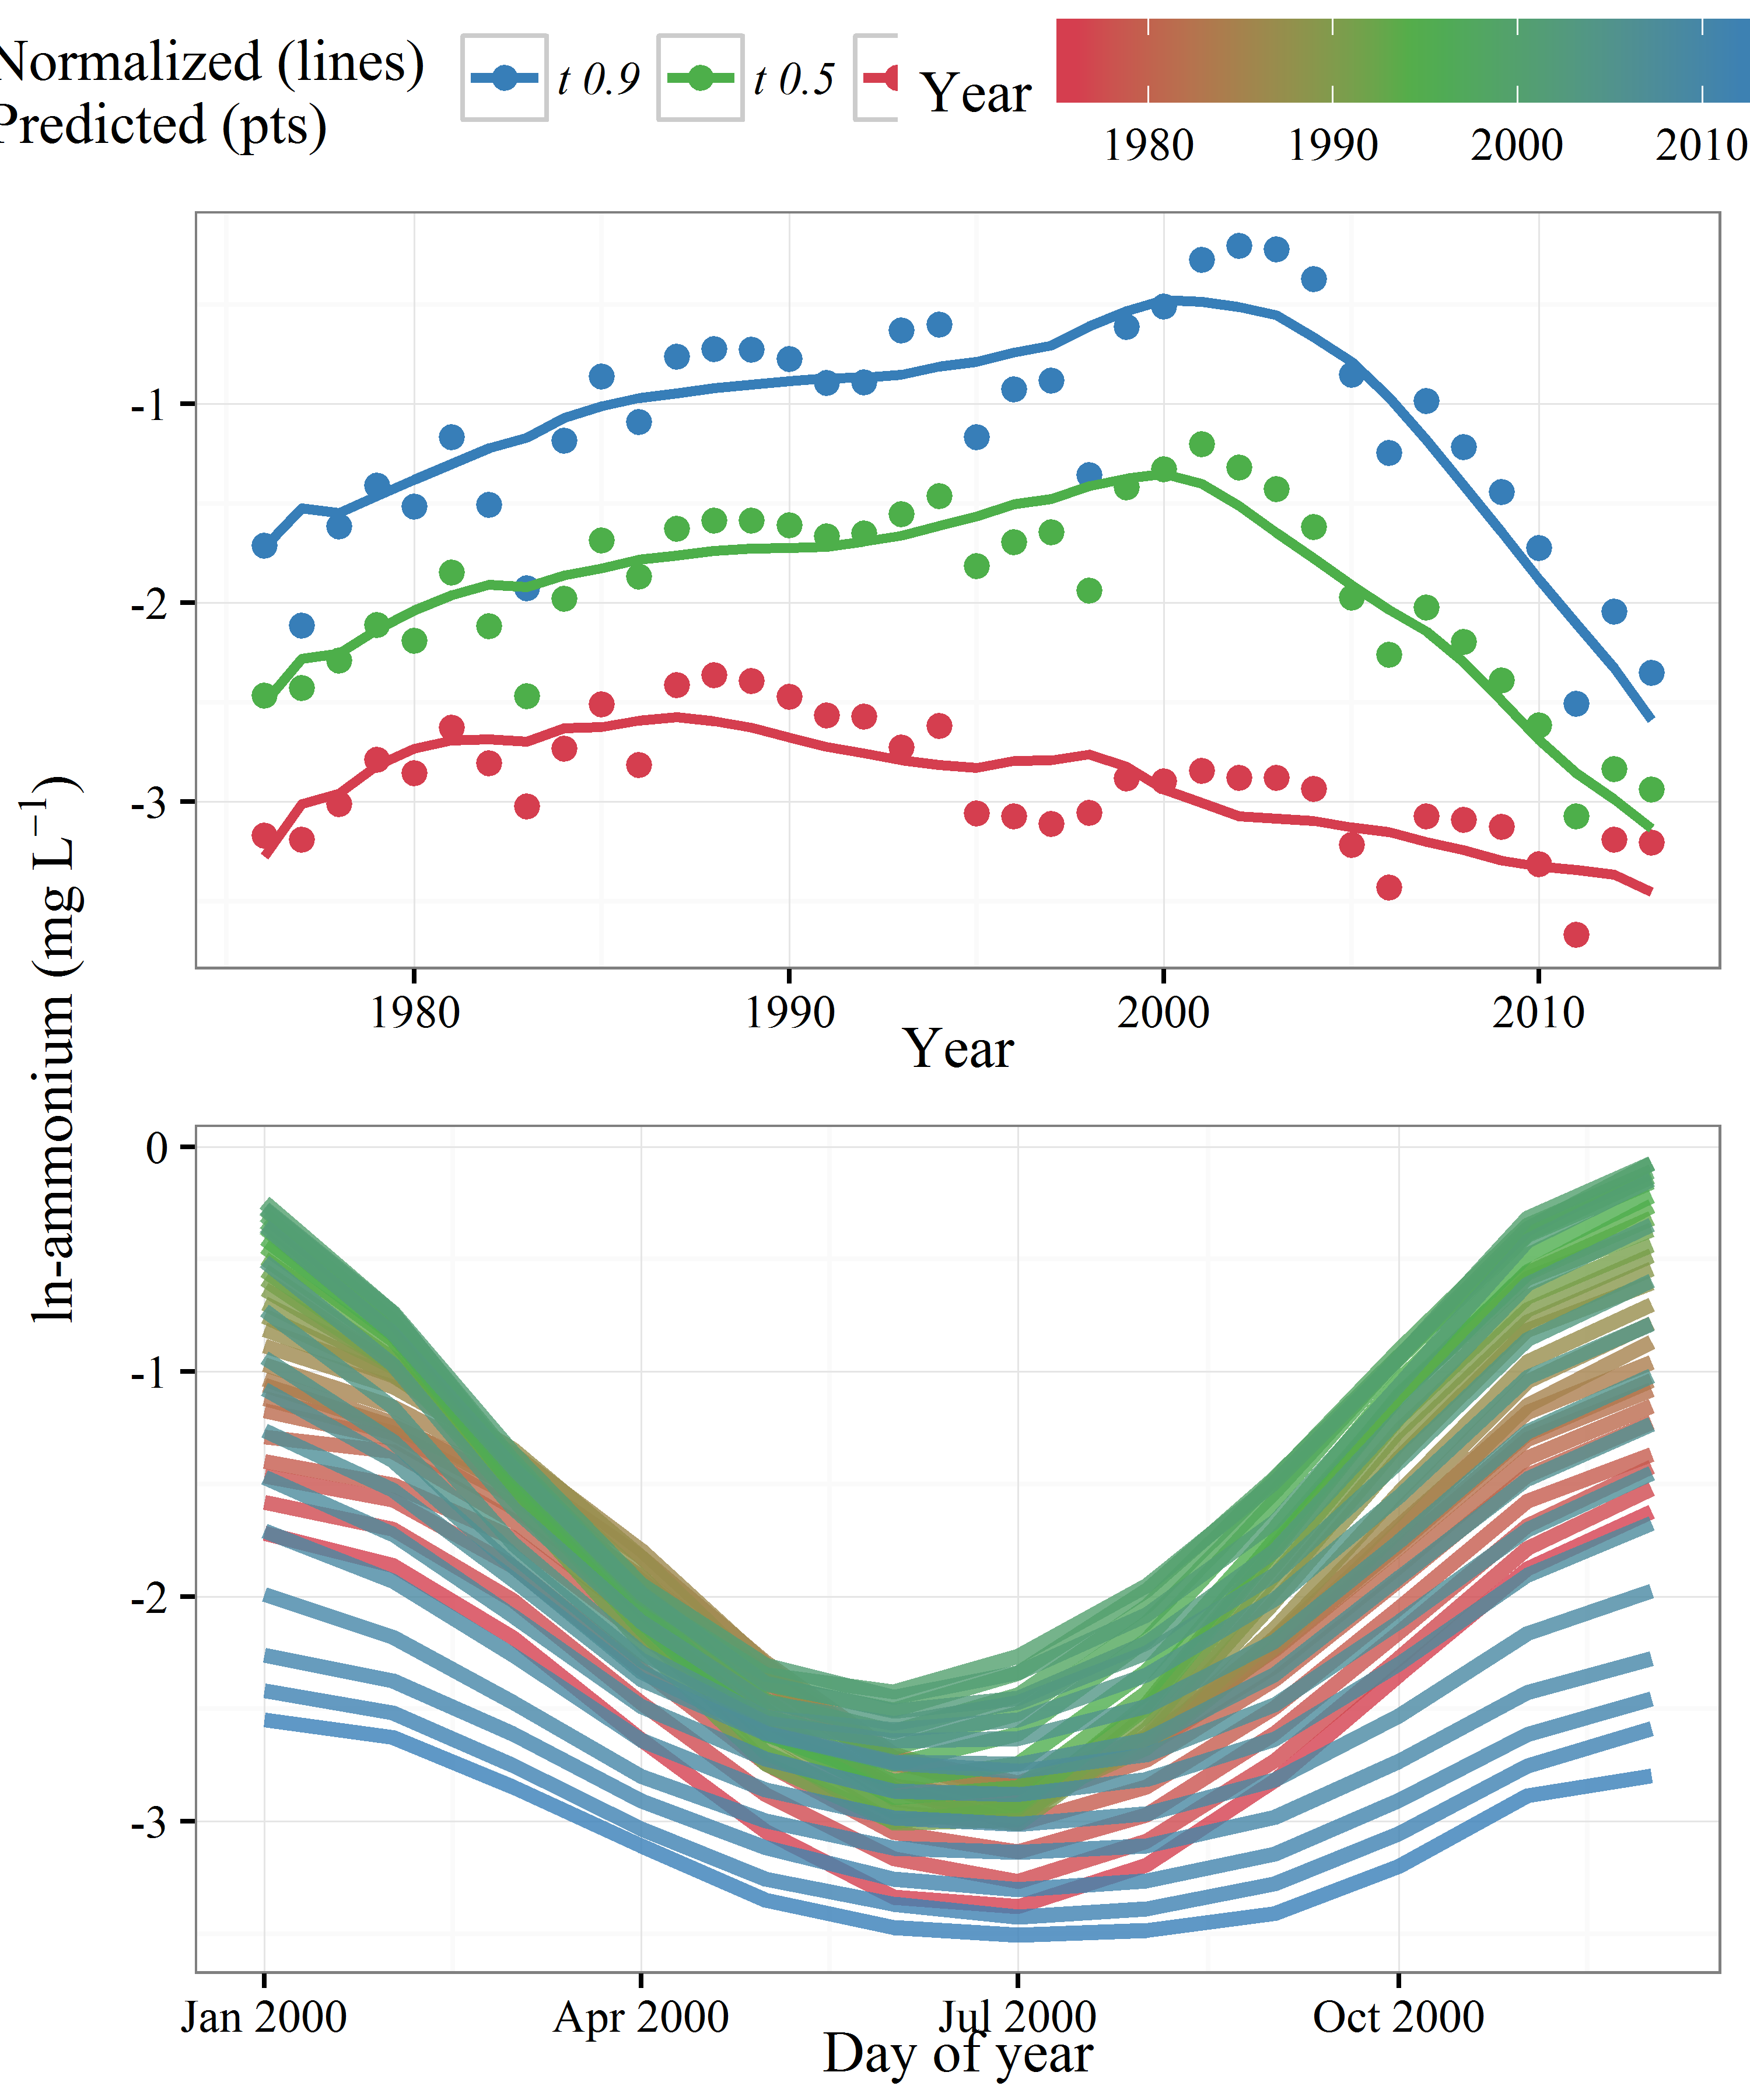
\includegraphics[width=\linewidth]{posterfigs/prdseas.png}}
        \caption{\footnotesize Examples of model results at P8 showing monthly and annual response to flow changes (top left), monthly quantile ($\tau$) distributions of flow-normalized predictions (bottom left), quantile distributions of annual trends (top right), and annual changes in seasonal variation (bottom right).}
	      \end{figure}		

	    \end{column}
	    
	    \end{columns}
	    \vspace{-1.75cm}
      \end{block}

   		%%%%%%
			% Trend analyses
			%%%%%%
			
% maps

			
      \begin{block}{Trend Analyses with WRTDS Results}
      Results for \alert{nine delta stations} and \alert{three nitrogen analytes} were used to evaluate \alert{annual and monthly trends} over time and space
      \vspace{-1.5cm}	
      \begin{columns}[t]
  
        %%
        \begin{column}{0.32\linewidth}
% table din
% latex table generated in R 3.2.3 by xtable 1.8-2 package
% Fri Apr 15 14:25:49 2016
\begin{table}[ht]
\centering
\caption{\footnotesize Percent changes in \alert{DIN} by years/months.} 
\begingroup\scriptsize
\begin{tabularx}{0.95\textwidth}{lRRRRRR}
  \toprule
Site & 1976-1988 & 1989-2000 & 2001-2012 & JFMA & MJJA & SOND \\ 
  \midrule
C10 & \it{\bf{\footnotesize 28.3}} & \it{\bf{\footnotesize 17.4}} & -41.7 & -25.7 & -10.1 & \it{\bf{\footnotesize 1.7}} \\ 
  C3 & \it{\bf{\footnotesize 23.9}} & \it{\bf{\footnotesize 26.8}} & -13.9 & \it{\bf{\footnotesize 30.7}} & \it{\bf{\footnotesize 54.8}} & \it{\bf{\footnotesize 42.8}} \\ 
  D19 & -19.8 & \it{\bf{\footnotesize 3.3}} & -15.3 & -28.6 & -35.1 & -15.6 \\ 
  D26 & -5.2 & \it{\bf{\footnotesize 10.9}} & -19.4 & -10.9 & -3.4 & -2.6 \\ 
  D28 & -21.7 & \it{\bf{\footnotesize 3.9}} & -37.3 & -32.9 & -53.3 & -48.8 \\ 
  D4 & -10.9 & \it{\bf{\footnotesize 20.3}} & -7.1 & \it{\bf{\footnotesize 11.4}} & \it{\bf{\footnotesize 4.8}} & \it{\bf{\footnotesize 10.7}} \\ 
  D6 & -7.4 & \it{\bf{\footnotesize 21.6}} & -8.5 & -4.7 & \it{\bf{\footnotesize 45.6}} & \it{\bf{\footnotesize 34.7}} \\ 
  D7 & -24.2 & \it{\bf{\footnotesize 17}} & -6.1 & -6.9 & \it{\bf{\footnotesize 19}} & \it{\bf{\footnotesize 21.4}} \\ 
  P8 & \it{\bf{\footnotesize 49.9}} & \it{\bf{\footnotesize 38.4}} & -35.7 & \it{\bf{\footnotesize 31.6}} & \it{\bf{\footnotesize 52.8}} & \it{\bf{\footnotesize 45.4}} \\ 
   \bottomrule
\end{tabularx}
\endgroup
\end{table}

    	    \vspace{-0.75cm}
    	    \begin{figure}
          \centerline{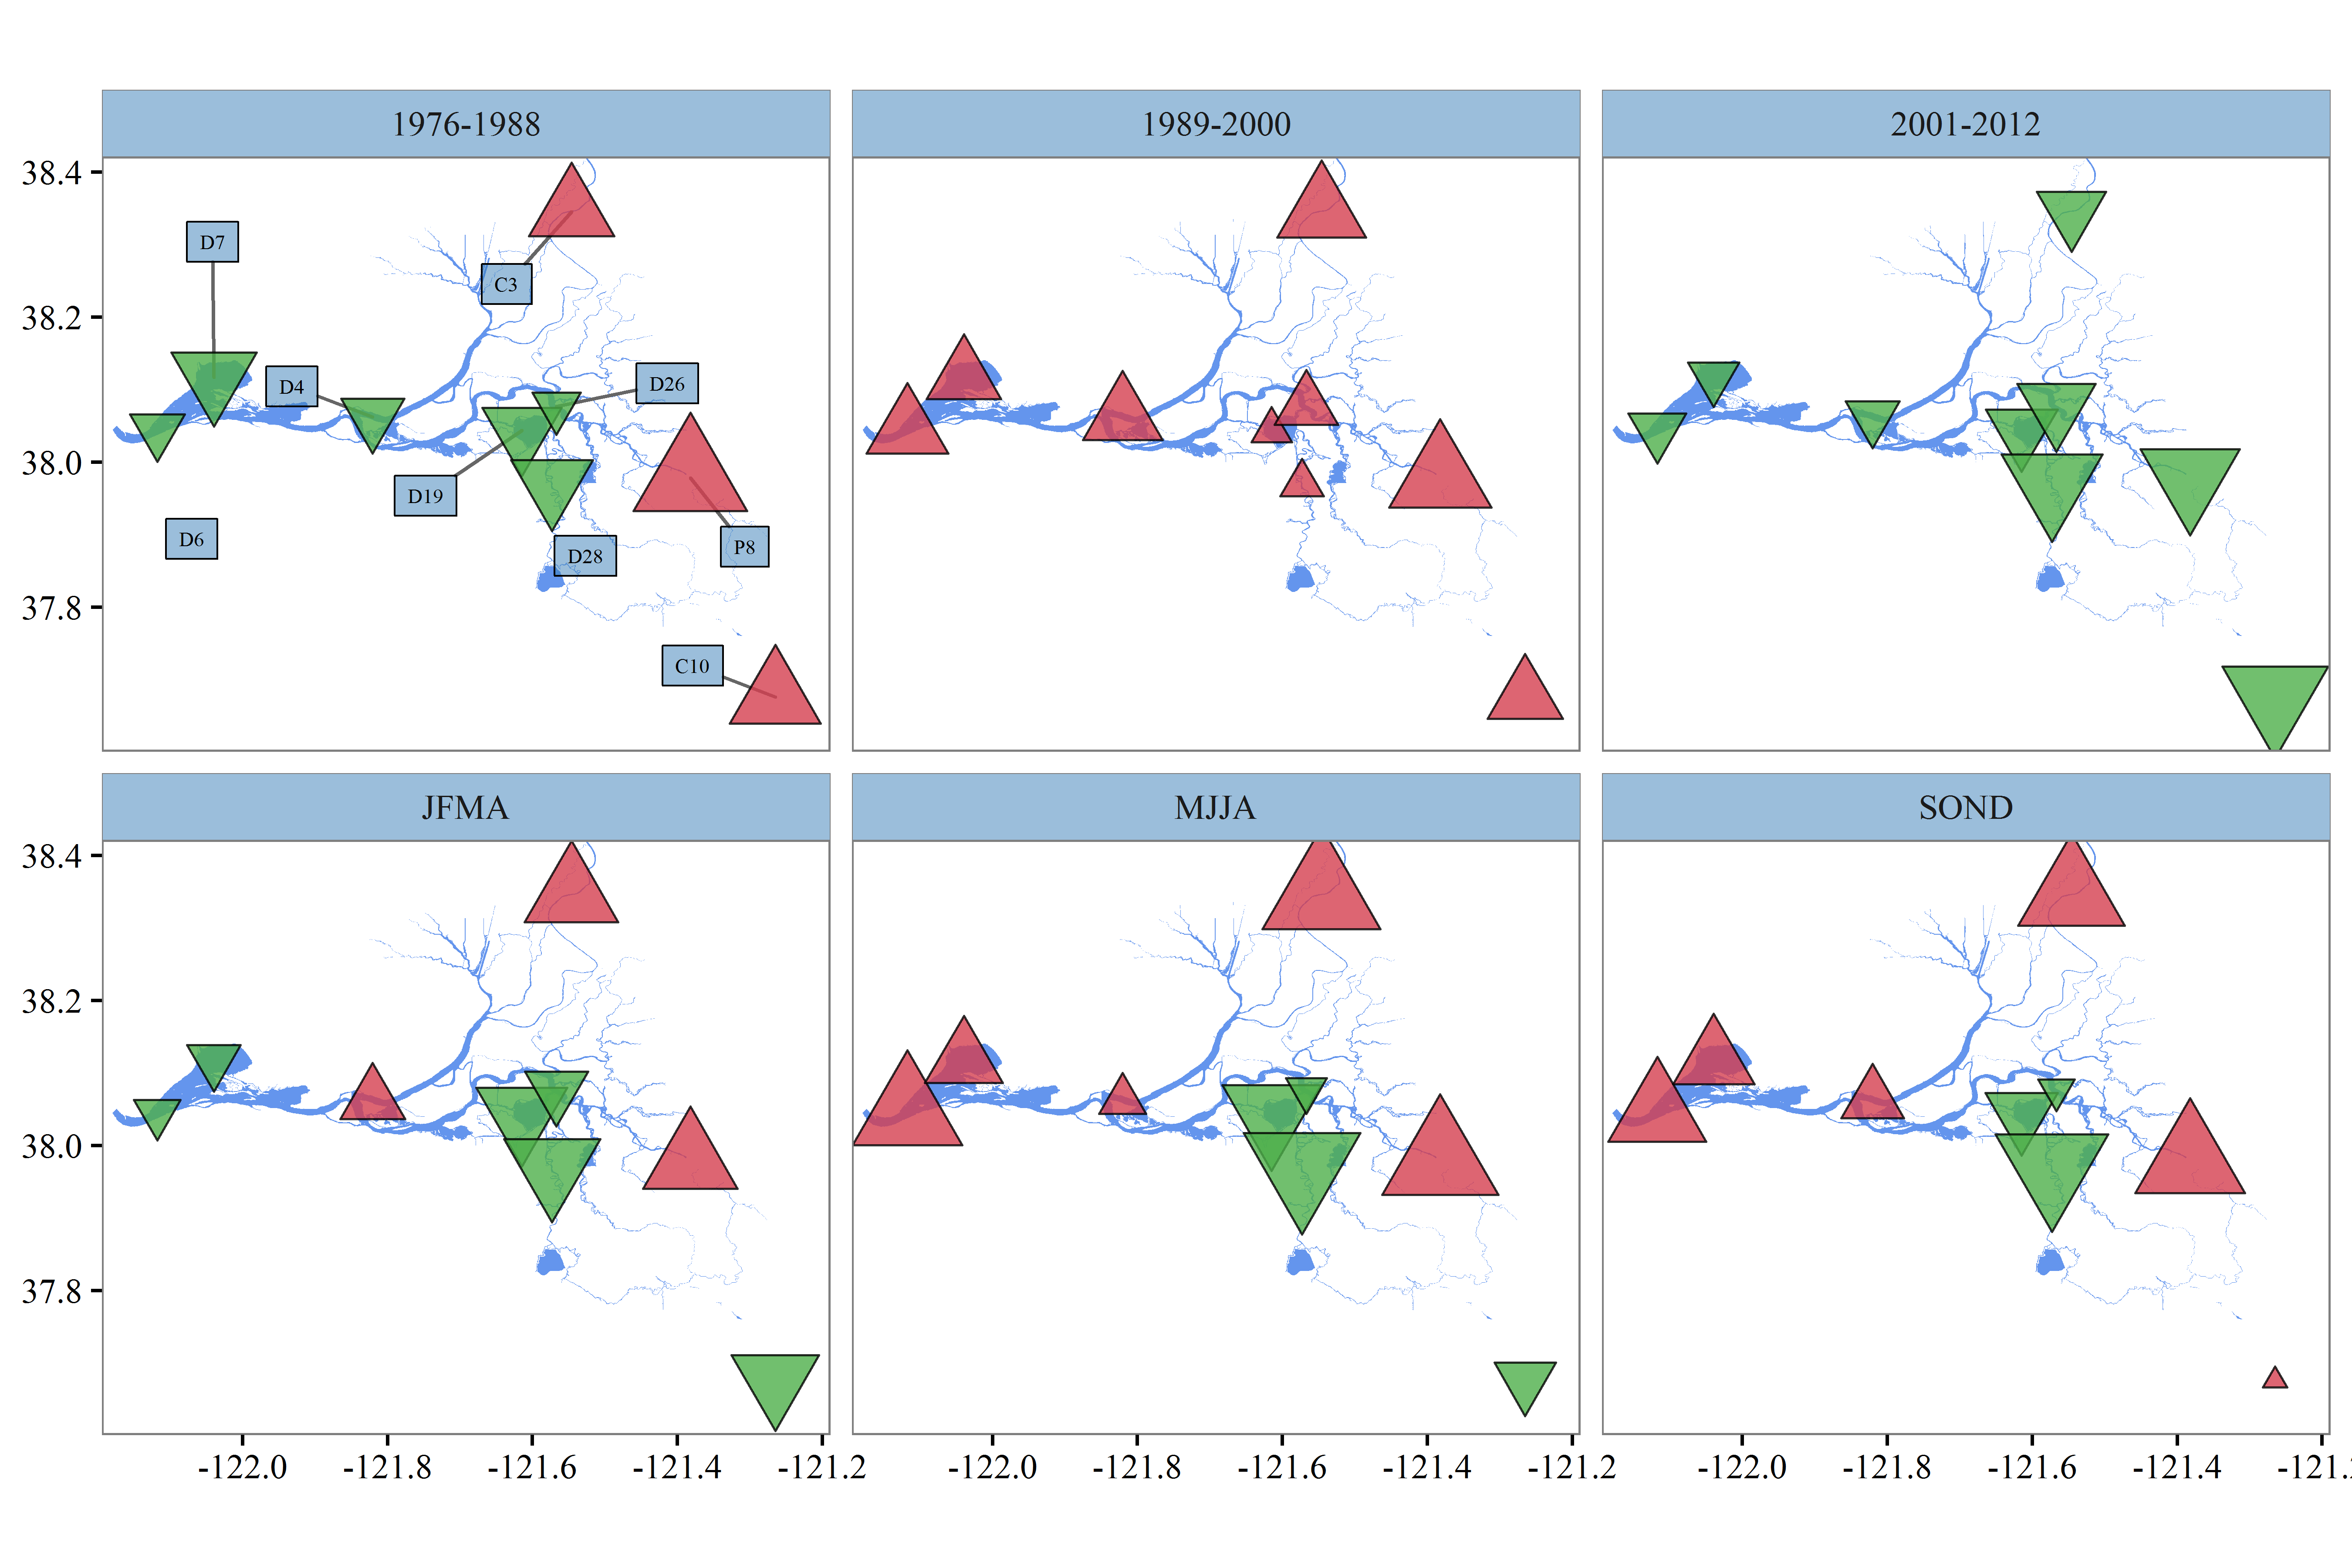
\includegraphics[width=\linewidth]{posterfigs/dinmap.png}}
    	    \end{figure}		
  	    \end{column}

        %%
        \begin{column}{0.32\linewidth}
% table nh4
% latex table generated in R 3.2.3 by xtable 1.8-2 package
% Fri Apr 15 14:25:49 2016
\begin{table}[ht]
\centering
\caption{\footnotesize Percent changes in \alert{ammonium} by years/months.} 
\begingroup\scriptsize
\begin{tabularx}{0.95\textwidth}{lRRRRRR}
  \toprule
Site & 1976-1988 & 1989-2000 & 2001-2012 & JFMA & MJJA & SOND \\ 
  \midrule
C10 & -39 & -54.1 & -46.5 & -77.1 & -88.7 & -90.9 \\ 
  C3 & \it{\bf{\footnotesize 53.6}} & \it{\bf{\footnotesize 41.6}} & -18.1 & \it{\bf{\footnotesize 81.8}} & \it{\bf{\footnotesize 95.8}} & \it{\bf{\footnotesize 74.6}} \\ 
  D19 & \it{\bf{\footnotesize 8.8}} & -5.6 & -7.5 & -16 & -21.8 & -4.8 \\ 
  D26 & \it{\bf{\footnotesize 22.8}} & \it{\bf{\footnotesize 8.4}} & -20.9 & -0.9 & \it{\bf{\footnotesize 7.9}} & \it{\bf{\footnotesize 18.7}} \\ 
  D28 & -11.8 & -16.9 & -18.2 & -42.3 & -24.7 & -34.7 \\ 
  D4 & \it{\bf{\footnotesize 5.3}} & \it{\bf{\footnotesize 46.8}} & -5.1 & \it{\bf{\footnotesize 66.9}} & \it{\bf{\footnotesize 33.6}} & \it{\bf{\footnotesize 68.3}} \\ 
  D6 & \it{\bf{\footnotesize 11.8}} & \it{\bf{\footnotesize 33}} & -9.7 & \it{\bf{\footnotesize 36}} & \it{\bf{\footnotesize 56.4}} & \it{\bf{\footnotesize 45.3}} \\ 
  D7 & -20.8 & \it{\bf{\footnotesize 25.2}} & -11.6 & \it{\bf{\footnotesize 21.2}} & -16 & \it{\bf{\footnotesize 34}} \\ 
  P8 & \it{\bf{\footnotesize 143.1}} & \it{\bf{\footnotesize 46.7}} & -86.5 & -52.7 & -23.9 & -61.1 \\ 
   \bottomrule
\end{tabularx}
\endgroup
\end{table}

    	    \vspace{-0.75cm}
    	    \begin{figure}
          \centerline{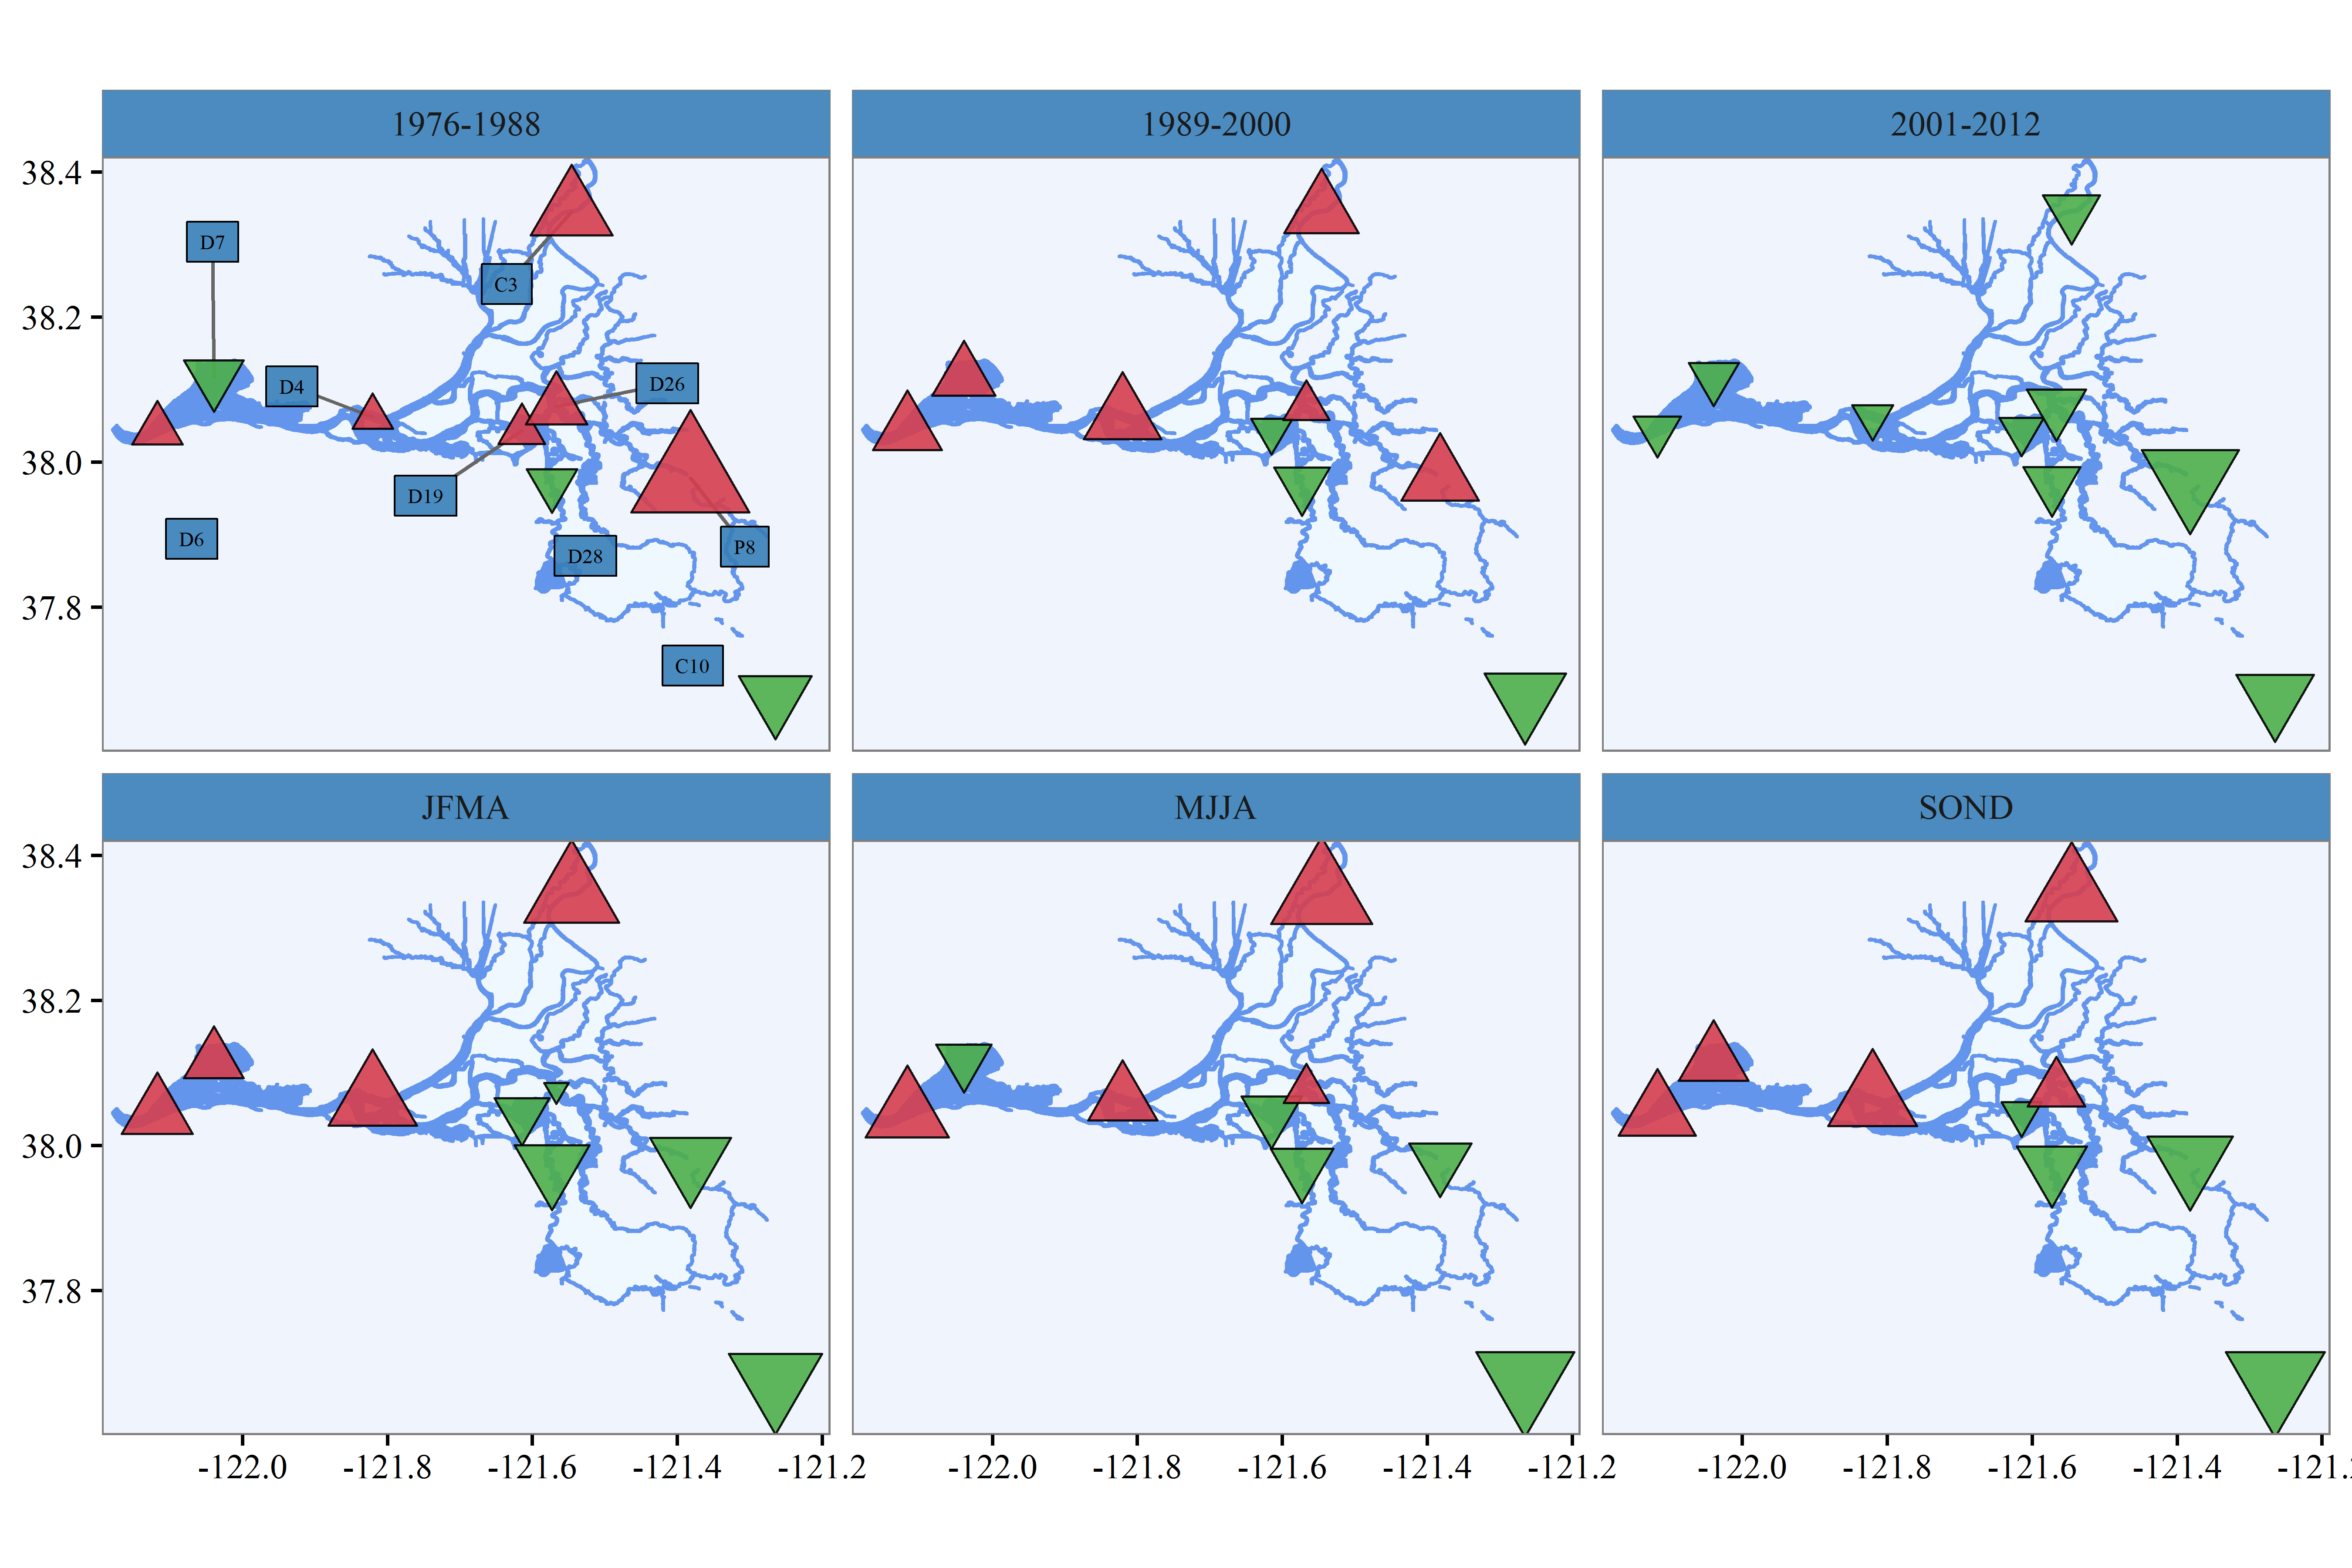
\includegraphics[width=\linewidth]{posterfigs/nh4map.png}}
    	    \end{figure}		
	      \end{column}
	    
	      %%
        \begin{column}{0.32\linewidth}
% table no23      
% latex table generated in R 3.2.3 by xtable 1.8-2 package
% Fri Apr 15 14:25:49 2016
\begin{table}[ht]
\centering
\caption{\footnotesize Percent changes in \alert{nitrite/nitrate} by years/months.} 
\begingroup\scriptsize
\begin{tabularx}{0.95\textwidth}{lRRRRRR}
  \toprule
Site & 1976-1988 & 1989-2000 & 2001-2012 & JFMA & MJJA & SOND \\ 
  \midrule
C10 & \it{\bf{\footnotesize 38.7}} & \it{\bf{\footnotesize 23.7}} & -40.8 & -12.5 & -0.2 & \it{\bf{\footnotesize 20.4}} \\ 
  C3 & -7.2 & \it{\bf{\footnotesize 11.9}} & -3.6 & -2.3 & \it{\bf{\footnotesize 29.4}} & \it{\bf{\footnotesize 3.3}} \\ 
  D19 & -21.8 & \it{\bf{\footnotesize 8.7}} & -16.5 & -28.6 & -34 & -16.3 \\ 
  D26 & -11 & \it{\bf{\footnotesize 12.9}} & -18.9 & -13.4 & -11.8 & -4.7 \\ 
  D28 & -30.2 & \it{\bf{\footnotesize 7.9}} & -39.1 & -34.5 & -59.1 & -53.8 \\ 
  D4 & -9.2 & \it{\bf{\footnotesize 15.9}} & -6.0 & \it{\bf{\footnotesize 5.4}} & \it{\bf{\footnotesize 6.6}} & \it{\bf{\footnotesize 7.3}} \\ 
  D6 & -7.8 & \it{\bf{\footnotesize 16.7}} & -8.8 & -17.9 & \it{\bf{\footnotesize 42.6}} & \it{\bf{\footnotesize 27.6}} \\ 
  D7 & -6 & \it{\bf{\footnotesize 18}} & -9.9 & -12.7 & \it{\bf{\footnotesize 41.9}} & \it{\bf{\footnotesize 24.4}} \\ 
  P8 & \it{\bf{\footnotesize 39.1}} & \it{\bf{\footnotesize 33.9}} & -18.8 & \it{\bf{\footnotesize 52.2}} & \it{\bf{\footnotesize 60.6}} & \it{\bf{\footnotesize 67.3}} \\ 
   \bottomrule
\end{tabularx}
\endgroup
\end{table}

    	    \vspace{-0.75cm}
    	    \begin{figure}
          \centerline{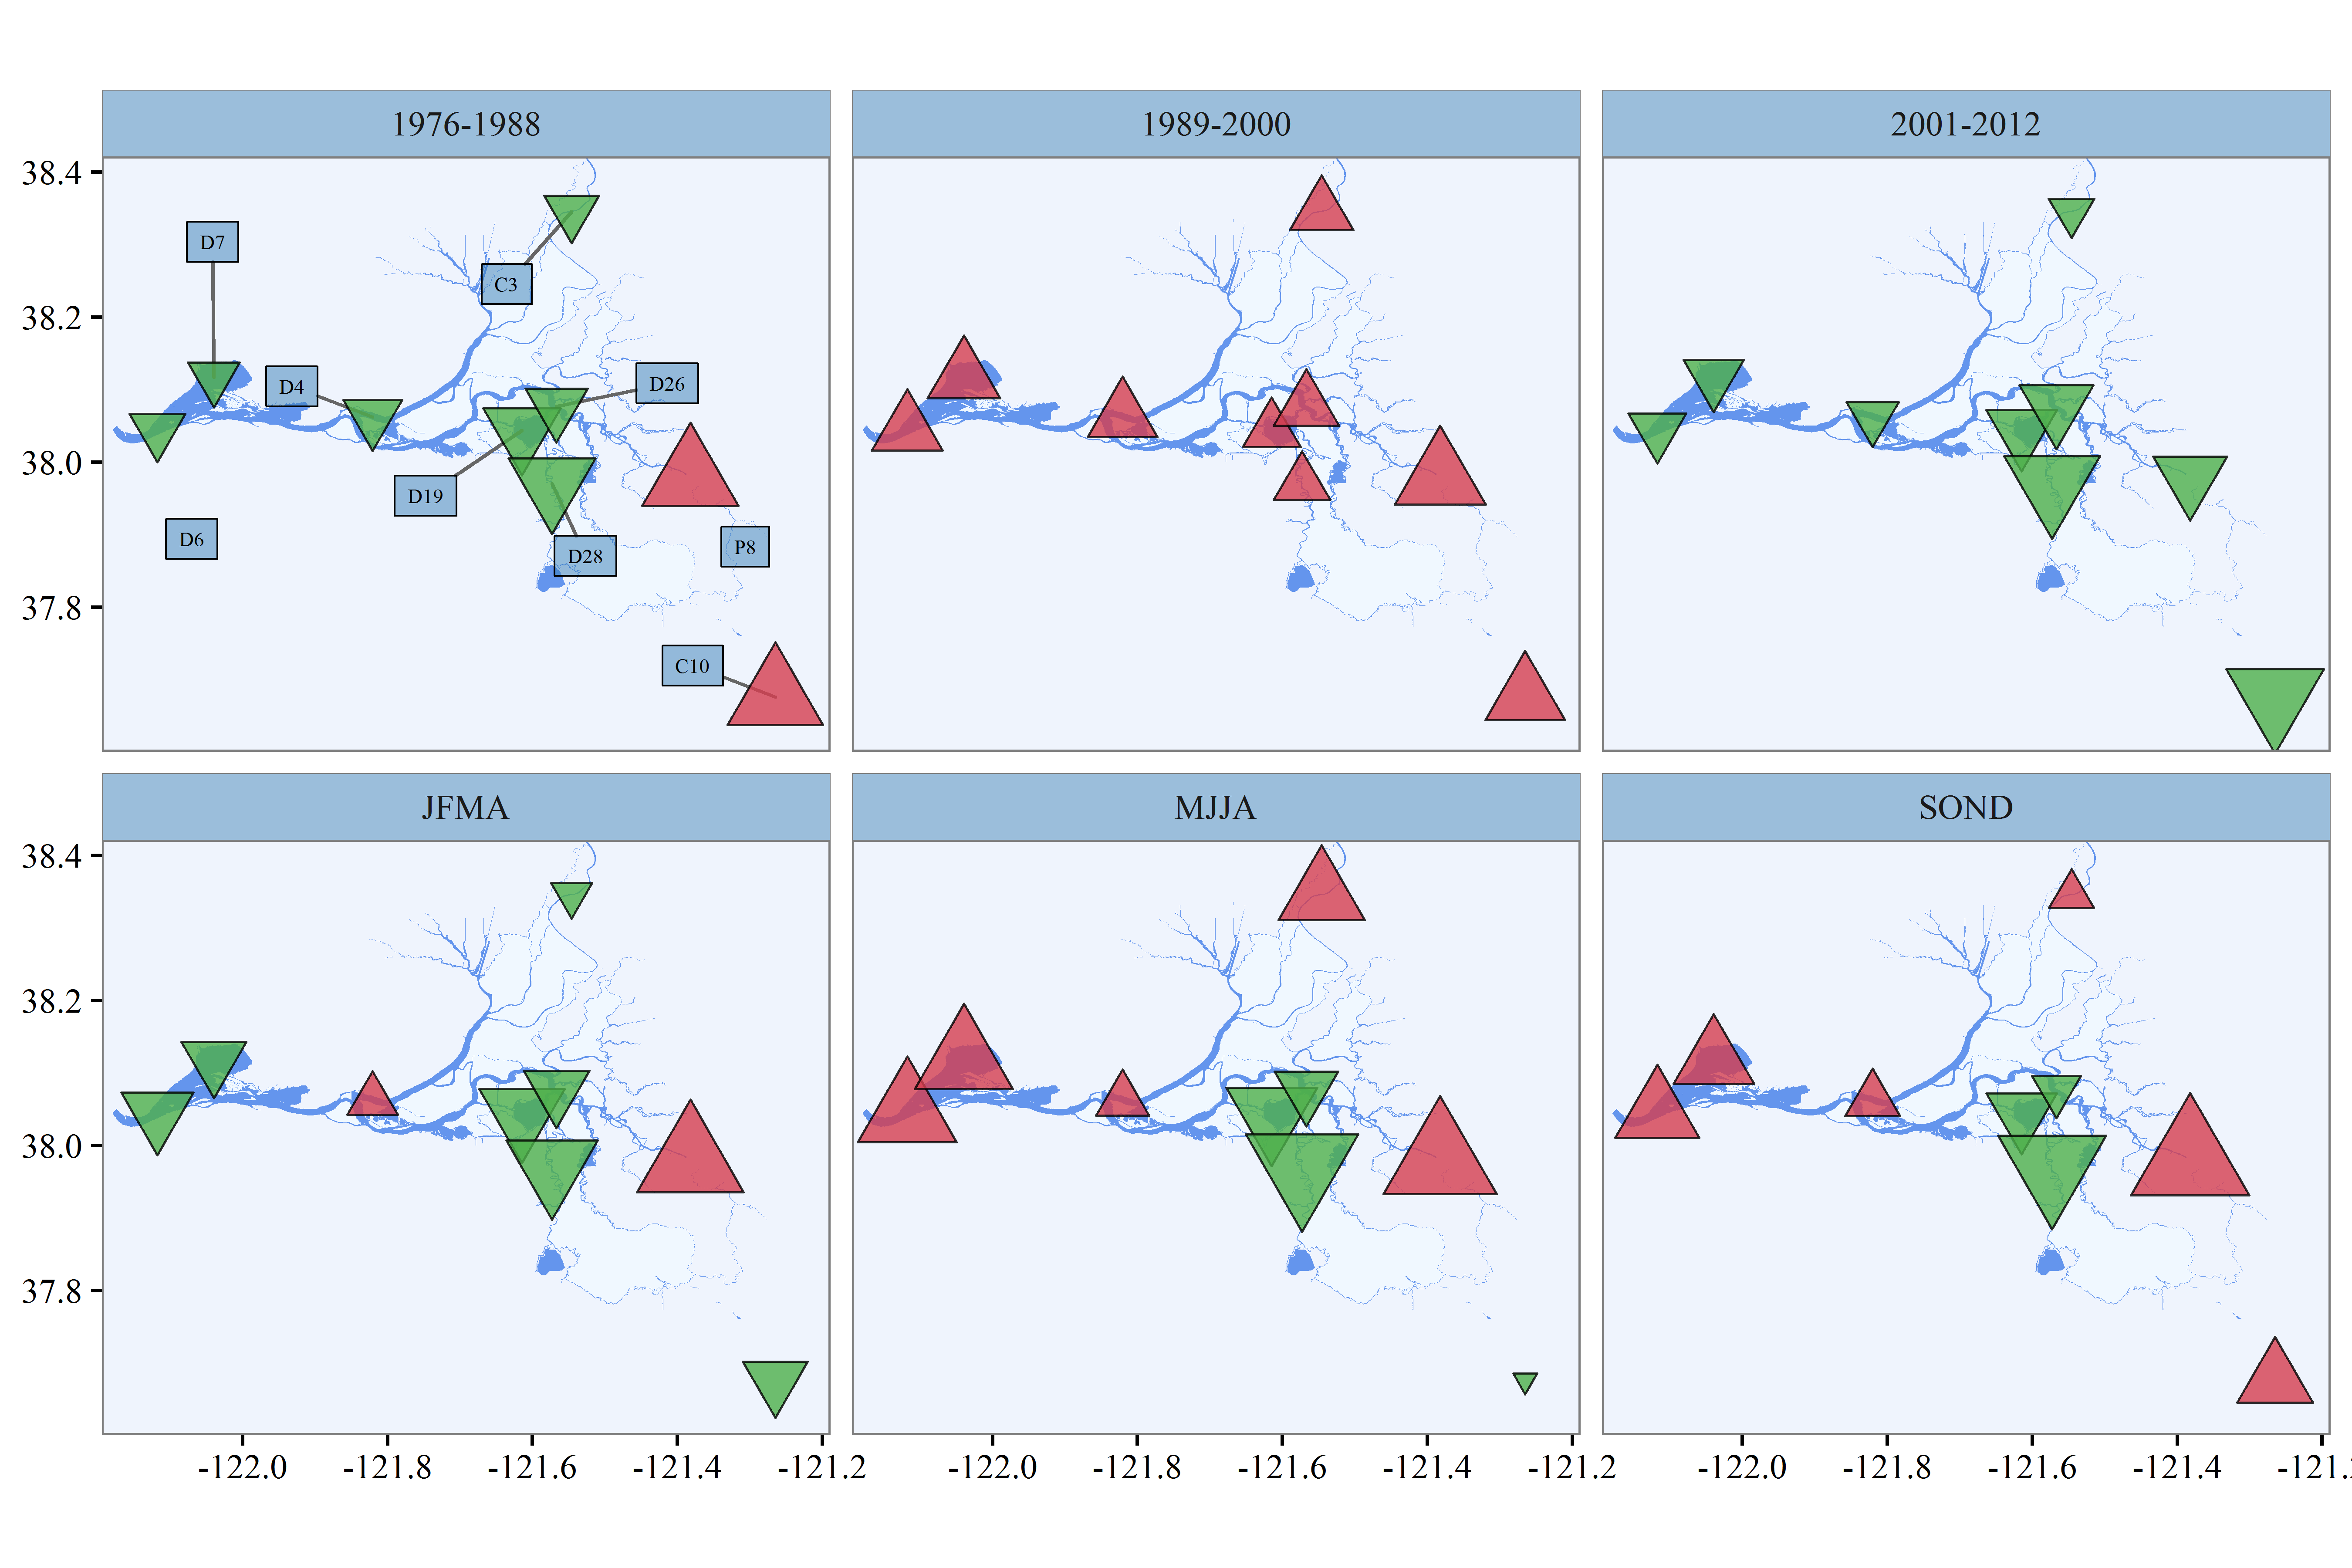
\includegraphics[width=\linewidth]{posterfigs/no23map.png}}
    	    \end{figure}		
	      \end{column}

	    \end{columns}
	    \vspace{-2.5cm}				
			\end{block}

    %%%%%%%%%%%%%%
  	% CENTER, RIGHT, BOTTOM BLOCKS
  	%%%%%%%%%%%%%%    
  	
      \vspace{-1.5cm}
      \begin{columns}[t, totalwidth=\linewidth]

        \begin{column}{.5\linewidth}
    
        \begin{varblock}[0.96\textwidth]{Evaluation of Additional Indicators}
          \alert{Covariation} among indicators can provide \alert{mechanistic clues}
          \begin{figure}
          \centerline{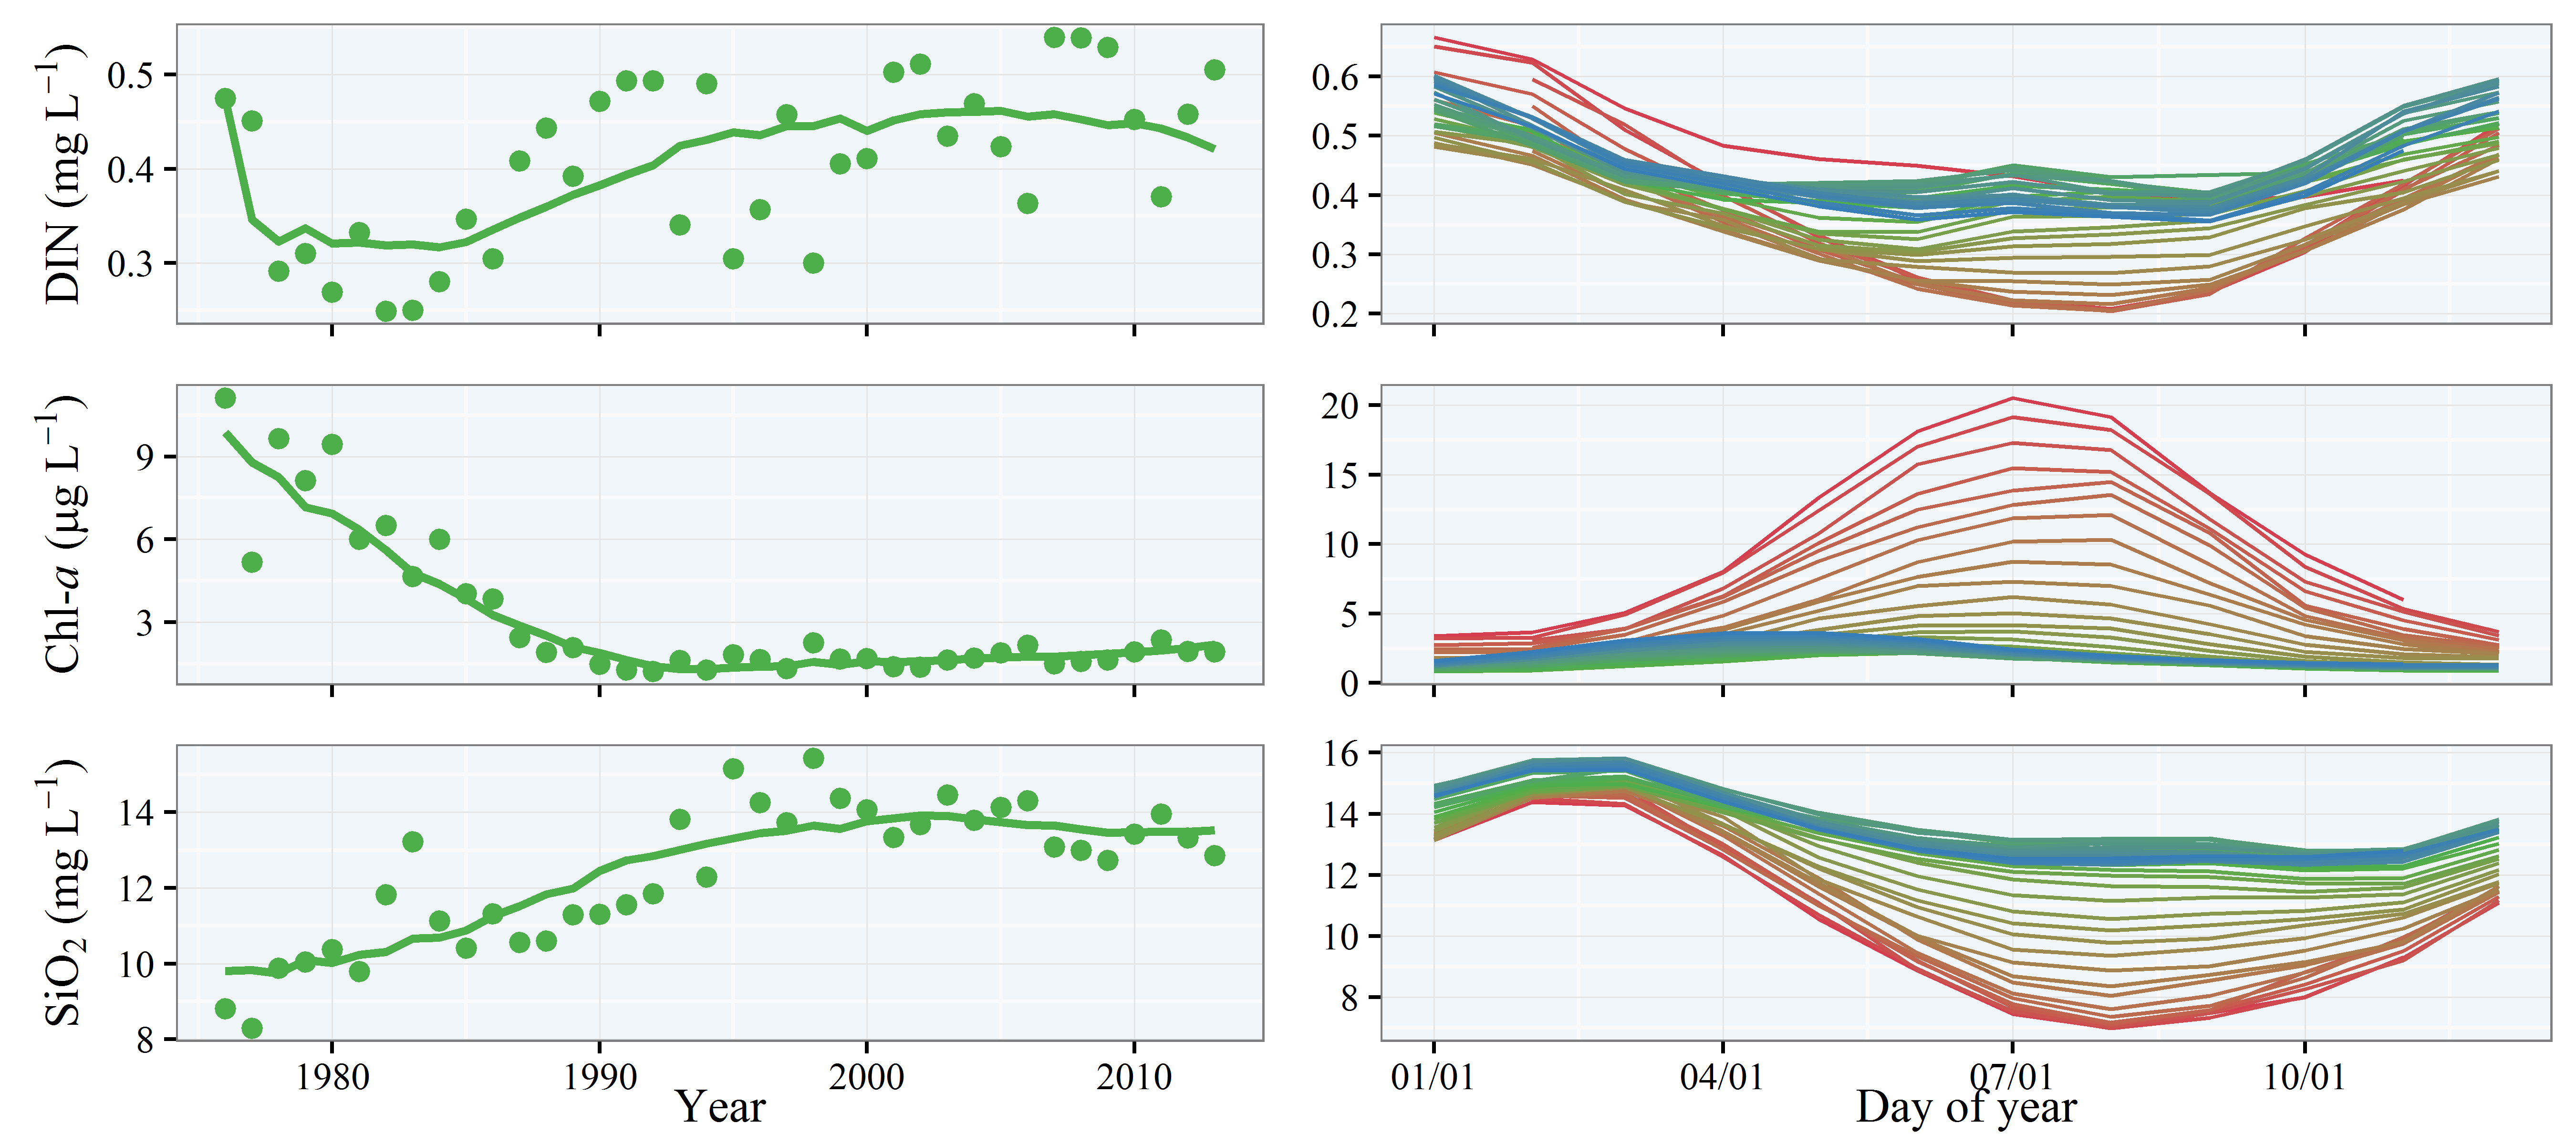
\includegraphics[width=0.95\linewidth]{posterfigs/d7trnds.png}}
          \caption{\footnotesize Flow-normalized trends of annual (left) and seasonal (right) variation in DIN, Chl-{\it\footnotesize a}, and SiO$_2$ at D7.  RGB colors indicate a unique year from 1976 to 2012 (see above).}
    	    \end{figure}	
    	    \vspace{-2.18cm}
    	  \end{varblock}
    
        \end{column}
        
        \begin{column}{.5\linewidth}
    
        \begin{varblock}[\textwidth]{Conclusions}
        \begin{itemize}
        \item WRTDS analyses on four decades of nutrient data revealed \alert{undescribed spatiotemporal variation}, e.g., large, nonmonotonic changes in NH$^{4+}$ at P8
        \item Trends among stations differed dramatically among \alert{different quantiles}, long term change was \alert{more dynamic in the upper quantiles}
        \item Long-term changes were observed in seasonal \alert{NH$^{4+}$ distributions}, eg., concentration \alert{reductions during winter}
        \end{itemize}
        \end{varblock}
        \small{
        We acknowledge the significant efforts of the California Department of Water Resources Environmental Monitoring Program in providing access to data. 
        
        Interactive data app of full results: https://beckmw.shinyapps.io/sf\_trends/
        
        WRTDStidal R package: https://github.com/fawda123/WRTDStidal
        }
        \end{column}
        
      \end{columns}
  
  
    %%  
    \end{column}
  
  \end{columns}
  
\end{frame}

\end{document}
